% 2018 浙江卷第21题：抛物线弦中点几何图
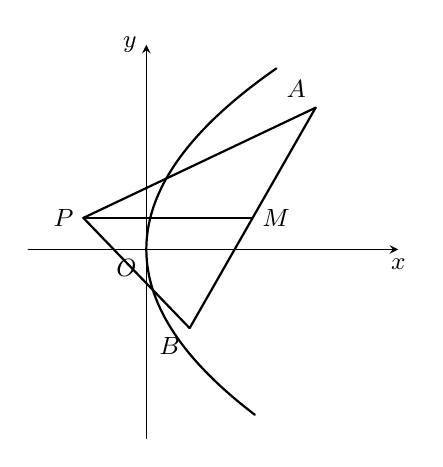
\begin{tikzpicture}[font=\small, line cap=round, line join=round, >=stealth, scale=1.0]
  % 坐标轴
  \draw[->] (-1.5, 0) -- (3.2, 0) node[below] {$x$};
  \draw[->] (0, -2.4) -- (0, 2.6) node[left] {$y$};
  \node[below left] at (0, 0) {$O$};

  % 抛物线 y^2 = 3.5x (示意)
  \draw[thick, domain=-2.1:2.3, samples=90] plot ({(\x)^2 / 3.2}, \x);

  % 关键点定义
  \coordinate (P) at (-0.8, 0.4);
  \coordinate (M) at (1.35, 0.4);
  \coordinate (A) at (2.15, 1.8);
  \coordinate (B) at (0.55, -1.0);

  % 连线
  \draw[thick] (P) -- (M);
  \draw[thick] (A) -- (B);
  \draw[thick] (P) -- (A);
  \draw[thick] (P) -- (B);

  % 标签
  \node[left] at (P) {$P$};
  \node[right] at (M) {$M$};
  \node[above left] at (A) {$A$};
  \node[below left] at (B) {$B$};
\end{tikzpicture}
